\documentclass[12pt]{scrartcl}

\usepackage[ngerman]{babel}
\usepackage[utf8]{inputenc}
\usepackage[T1]{fontenc}

\usepackage{fancyhdr}
\usepackage{enumerate}
\usepackage{amssymb}
\usepackage{mathtools}

\usepackage{graphicx}
\usepackage[dot, phantomtext]{dashundergaps}
\usepackage[shortlabels]{enumitem}
\usepackage{wasysym}
\usepackage{multicol}
\usepackage{xcolor}
\usepackage{tikz}
\usepackage{pgf}
\usepackage{tikz}

\parindent 0em

\fancyhf{}
\pagestyle{fancy}

\fancyhead[L]{Name:\hspace{8cm}Student number:}
\fancyfoot[R]{Page \thepage}

\fancypagestyle{firststyle}
{
	 \renewcommand{\headrulewidth}{0pt}%
   \fancyhf{}%
   \fancyfoot[R]{Page \thepage}
}

\allowdisplaybreaks

\begin{document}

\thispagestyle{firststyle}

\begin{center}
\large{Exam}\\
%\large{Exam}\\
\vspace{0.5cm}
\large{\textbf{"`Introduction to Digital Work"'}}\\
\vspace{0.5cm}
\large{Prof. Dr. Gerit Wagner}\\
\vspace{0.5cm}
\large{Test exam}\\
\end{center}
\vspace{3cm}

Please note:
\begin{itemize}
\item The exam consists of 5 (five) parts, and you have 90 Minutes to complete it.
\item You can score 90 points overall (you have 1 minute for each point).
\item It is mandatory to use a pen with black or blue color. Anything written with a pencil will not be graded.
\item Points earned as part of the bonus exercises will be added to your score.
\item Auxiliaries: Dictionary (without annotations).
\end{itemize}
\vspace{2cm}


\vfill

\clearpage

\subsection*{Part 1: Drivers of change in digital work (15 Points)}

\textbf{A (7 points)} Indicate whether the following statements are true or false. (\textit{You receive points for correct answers and deductions for incorrect ones.})

\begin{description}

	\item[Statement 1] In digital work, research findings generally apply across different types of organizations.

	\begin{multicols}{2}
		\begin{itemize}[label={\Square}]
			\item True
			\item False
		\end{itemize}
	\end{multicols}

	\item[Statement 2] Cal Newport suggests that graduates looking for a job should always follow their passion.
	
	\begin{multicols}{2}
		\begin{itemize}[label={\Square}]
			\item True
			\item False
		\end{itemize}
	\end{multicols}

	\item[Statement 3] The \textit{war for talent} allows highly qualified graduates to demand more flexible work arrangements, including remote work.

	\begin{multicols}{2}
		\begin{itemize}[label={\Square}]
			\item True
			\item False
		\end{itemize}
	\end{multicols}

	\item[Statement 4] Based on the hierarchy of evidence, data from an experiment should be considered as high-quality evidence, and data from an expert panel should be considered low-quality evidence.

	\begin{multicols}{2}
		\begin{itemize}[label={\Square}]
			\item True
			\item False
		\end{itemize}
	\end{multicols}

	\item[Statement 5] The \textit{New Work} paradigm assumes that workers have limited autonomy when reacting to the transformation of their work environments.

	\begin{multicols}{2}
		\begin{itemize}[label={\Square}]
			\item True
			\item False
		\end{itemize}
	\end{multicols}

	\item[Statement 6] Taylorism is a contemporary approach, which involves flat hierarchies.

	\begin{multicols}{2}
		\begin{itemize}[label={\Square}]
			\item True
			\item False
		\end{itemize}
	\end{multicols}

	\item[Statement 7 ] Raj Chetty's data suggest that upward mobility is declining in the US.

	\begin{multicols}{2}
		\begin{itemize}[label={\Square}]
			\item True
			\item False
		\end{itemize}
	\end{multicols}

\end{description}

\textbf{B (8 points)} We considered different stages in the evolution of organizations, including the industrial and the digital revolution. Briefly summarize how these key stages affect the nature of work.

\subsection*{Part 2: Digital work individually (20 Points)}

\textbf{A (5 points)} Summarize the key categories of skills of the DigComp framework.

\vspace{0.3cm}

\textbf{B (5 points)} State the five core processes of Getting-Things-Done.

\vspace{0.3cm}
\textbf{C (10 points)} Your colleagues at work are skeptical about Getting-Things-Done because it has not been tested scientifically. You agree with them, but you also remember that this method aligns with established principles from cognitive research. Select two principles and explain how they are implemented in Getting-Things-Done.
 
\vspace{0.3cm}

\subsection*{Part 3: Digital work in teams (30 Points)}

\textbf{A (6 points)} In the case of Gitlab, we focused on a remote-first organization. Briefly summarize three of Gitlab's main principles for managing remote teams.

\vspace{0.3cm}

\textbf{B (8 points)} Your new colleague sends you a message informing you that he prefers to do all communication via Zoom. First, select and briefly outline a key benefit of using video conferences for communication. Afterward, highlight a situation in which e-mails could be preferred. Connect your position to prior theory.

\vspace{0.3cm}

\textbf{C (6 points)} Your team works with git. In your repository, you have completed the following operations. Which changes are in the commit? Which changes are staged? Which changes are unstaged?

\begin{verbatim}
# modify README.md, src/utils.py, docs/setup.rst
git add .
git restore --staged README.md
# modify README.md and docs/setup.rst
git restore README.md
git commit
\end{verbatim}
\vspace{0.3cm}

\newpage

\textbf{E (6 points)} Create the following git graph by using the short commands of the \textit{learngitbranching} tutorial (git commit, git checkout -b).

\vspace{1cm}
\begin{center}
	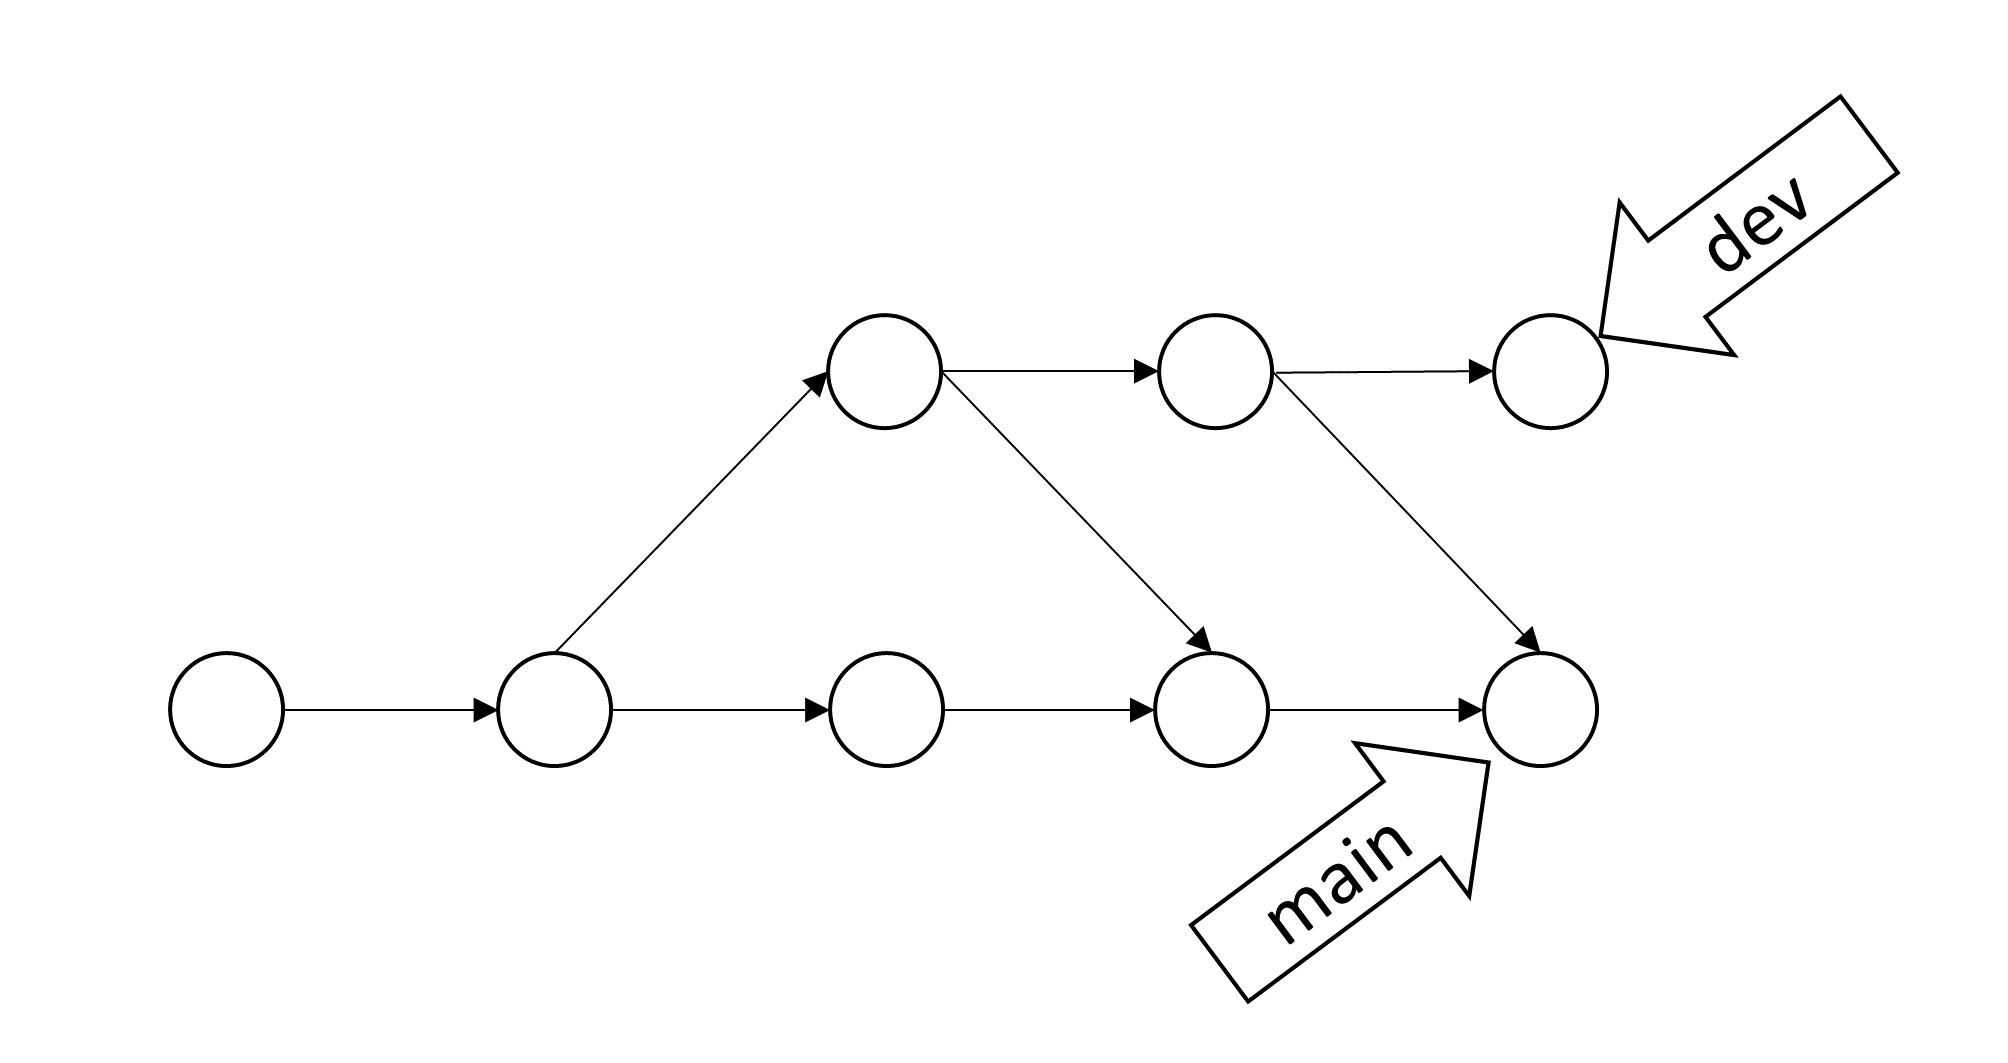
\includegraphics[scale=0.6]{git-graph_2.png}
\end{center}

\vspace{0.3cm}

\textbf{F (4 points)} Describe two challenges in Open-Source projects and potential measures to overcome them.

\subsection*{Part 4: Digital work in crowds (15 Points)}

\textbf{A (8 points)} Describe four possible ways in which digital entrepreneurs could use digital platforms, and provide an example for each one.

\vspace{0.3cm}

\textbf{B (7 points)} You are part of a campaign aimed at informing digital entrepreneurs about the potential challenges of working on platforms. Based on the work of Cutolo and Kenney (2021), draft a short summary of two significant challenges and two possible responses.

\subsection*{Part 5: Future of work (10 Points)}

\textbf{A (6 points)} Give three skills that are unlikely to be replaced by artificial intelligence and provide an illustrative example for each one.

\vspace{0.3cm}
\newpage
\textbf{B (4 points)} Indicate whether the following statements are true or false. (\textit{You receive points for correct answers and deductions for incorrect ones.})
\\
\begin{description}
	\item[Statement 1] Deontological approaches, such as Kant's categorical imperative, do not involve consideration of the potential consequences that a decision could have in a given situation.

\begin{multicols}{2}
	\begin{itemize}[label={\Square}]
		\item True
		\item False
	\end{itemize}
\end{multicols}

\item[Statement 2] Decisions based on utilitarian ethics could accept suffering of individuals when many others benefit.

\begin{multicols}{2}
	\begin{itemize}[label={\Square}]
		\item True
		\item False
	\end{itemize}
\end{multicols}

\item[Statement 3] Economic considerations related to the benefits and costs (potential harms) of workplace technology are rooted in Deontological ethics.

\begin{multicols}{2}
	\begin{itemize}[label={\Square}]
		\item True
		\item False
	\end{itemize}
\end{multicols}

\item[Statement 4] Jeremy Bentham's Panopticon is an utilitarian attempt to organize and justify surveillance.

\begin{multicols}{2}
	\begin{itemize}[label={\Square}]
		\item True
		\item False
	\end{itemize}
\end{multicols}

\end{description}

\end{document}
